% TAORG / V-HPED paper draft.
% Every number comes from paper/generated/ (scripts/make_paper_artifacts.py).
% Do not type result numbers by hand (Phases.md Phase 9).
\documentclass[10pt]{article}
\usepackage[margin=1in]{geometry}
\usepackage{amsmath,amssymb,amsthm}
\usepackage{booktabs}
\usepackage{graphicx}
\usepackage{xcolor}
\usepackage{algorithm}
\usepackage{algpseudocode}
\usepackage[hidelinks]{hyperref}
\usepackage{tikz}
\usetikzlibrary{positioning,arrows.meta}

\newtheorem{proposition}{Proposition}
\newtheorem{lemma}{Lemma}
\newtheorem{theorem}{Theorem}
\newcommand{\todo}[1]{\textcolor{red}{[TODO: #1]}}
\newcommand{\softplus}{\operatorname{softplus}}

% Generated by scripts/make_paper_artifacts.py - do not edit.
\newcommand{\synFullFrameFone}{0.958}
\newcommand{\synFullDelay}{3.37}
\newcommand{\synFullPersFone}{0.951}
\newcommand{\synFullFalsePers}{0.077}
\newcommand{\synFullECE}{0.030}
\newcommand{\synGatedFrameFone}{0.950}
\newcommand{\synGatedDelay}{5.05}
\newcommand{\synGatedPersFone}{0.922}
\newcommand{\synGatedFalsePers}{0.105}
\newcommand{\synGatedECE}{0.286}
\newcommand{\synVthmmFrameFone}{0.969}
\newcommand{\synVthmmDelay}{5.26}
\newcommand{\synVthmmPersFone}{0.951}
\newcommand{\synVthmmFalsePers}{0.089}
\newcommand{\synVthmmECE}{0.054}
\newcommand{\synNovisFrameFone}{0.922}
\newcommand{\synNovisDelay}{3.92}
\newcommand{\synNovisPersFone}{0.571}
\newcommand{\synNovisFalsePers}{0.080}
\newcommand{\synNovisECE}{0.060}
\newcommand{\synLazyexactFrameFone}{0.956}
\newcommand{\synLazyexactDelay}{3.63}
\newcommand{\synLazyexactPersFone}{0.948}
\newcommand{\synLazyexactFalsePers}{0.075}
\newcommand{\synLazyexactECE}{0.030}
\newcommand{\synSeeds}{5}
\newcommand{\synRunId}{20261027\_202753\_a7314fe5}
\newcommand{\cxMaxPairs}{3000}
\newcommand{\cxSpeedupSparse}{4.5}
\newcommand{\cxFracSparse}{0.05}
\newcommand{\cxSpeedupDense}{0.77}
\newcommand{\cxMismatches}{0}
\newcommand{\cxMachine}{Windows-10-10.0.26300-SP0}
\newcommand{\pilotAvailable}{0}


\title{Is It Gone or Just Hidden? Visibility-Thinned Hawkes Dynamics for\\
Persistent Relationships in Video Scene Graphs}
\author{TAORG team \todo{authors and affiliations}}
\date{Draft --- \today}

\begin{document}
\maketitle

\begin{abstract}
Video scene graph generators predict subject--predicate--object relationships
frame by frame, so a relationship that is briefly occluded or missed by the
detector flickers in and out of the output. Temporal smoothing hides the
flicker but also keeps relationships alive after they have really ended,
because it cannot tell \emph{why} an edge stopped being observed. We propose
V-HPED, a model-agnostic post-processing layer that treats the base model's
detections of a live relationship as a multivariate Hawkes process thinned
by visibility, and filters a latent alive/dead state with the exact
forward-algorithm likelihood. This gives visible absence a principled
meaning: its evidence against the relationship is proportional to the
current Hawkes intensity, so densely observed relationships are dropped
quickly when they disappear in plain view while occluded ones are carried
through. A cross-predicate hazard lets one predicate signal the end of
another. On the data-structure side we prove that, under two explicit
conditions, untouched edges evolve in closed form, which yields an exact
lazy implementation with a per-pair wake-up heap whose decisions match the
eager reference. In a controlled synthetic study with \synSeeds{} predeclared
seeds, fitted V-HPED drops terminated relationships after
\synFullDelay{} frames on average versus \synGatedDelay{} for
visibility-gated EMA, with better-calibrated alive probabilities.
Under synthetic ID switches, however, fitted V-HPED has lower frame F1 than visibility-gated EMA and is poorly calibrated.
Real-data evaluation on Action Genome is
\todo{pending --- pipeline ready, see Sec.~\ref{sec:pilot}}.
\end{abstract}

\section{Introduction}
Video scene graph generation (VidSGG) methods such as
STTran~\cite{cong2021sttran}, DSG-DETR~\cite{feng2023dsgdetr} and
TEMPURA~\cite{nag2023tempura} output, at each frame, a set of
relationship triplets between tracked objects. Downstream consumers need
relationship \emph{state}: is the person still holding the cup? Frame-wise
outputs answer this poorly. Occlusion, missed detections and tracker
failures~\cite{zhang2022bytetrack} make continuing relationships disappear
for a few frames, producing churn
(\texttt{holding} $\to$ missing $\to$ \texttt{holding}).

A temporal memory bridges such gaps, but every fixed-decay memory faces the
same trade-off: slow decay persists through occlusion and also through true
termination; fast decay does the opposite. The missing ingredient is the
\emph{reason} for absence. When an object is occluded, absence is censored
evidence; when both objects are clearly visible and the relationship is not
detected, absence is evidence that it ended --- and how strong that evidence
is should depend on how reliably this relationship has been detected so far.

\paragraph{Contributions.}
\begin{enumerate}
\item A \textbf{visibility-thinned Hawkes observation model} for VidSGG edge
persistence: detections of a live relationship form a multivariate Hawkes
process~\cite{hawkes1971spectra} thinned by visibility~\cite{lewis1979thinning};
a two-state alive/dead chain is filtered with the exact forward
likelihood~\cite{rabiner1989hmm}. Visible absence is \emph{not} treated as
a Hawkes event; its evidence follows from the thinned compensator
(Proposition~\ref{prop:evidence}).
\item A \textbf{cross-predicate termination hazard} that lets one predicate
(e.g.\ \texttt{putting down}) raise the hazard of another (\texttt{holding}).
\item \textbf{Exact lazy evaluation} with a per-pair wake-up heap, its
correctness proof and complexity, and a randomized equivalence harness
against the eager oracle (Sec.~\ref{sec:lazy}).
\item A \textbf{reproducible evaluation protocol}: deterministic corruption
manifests, frozen persistence/termination/churn/calibration metrics,
validation-only threshold selection and paired statistics.
\end{enumerate}
We do not claim to invent Hawkes processes, HMMs or thinning; the
contribution is their combination as an observation model for relationship
persistence, its exact likelihood and its efficient maintenance.

\section{Related work}
\paragraph{Video scene graphs.} Action Genome~\cite{ji2020actiongenome}
annotates person--object relationships on sampled frames. STTran, DSG-DETR
and TEMPURA model temporal context inside the network; our layer is
post-hoc and model-agnostic. \todo{verify closest occlusion-aware VidSGG
work and whether it is reproducible (PRD §11).}
\paragraph{Temporal point processes on graphs.} Hawkes processes with
nonlinear links~\cite{mei2017neuralhawkes} have been used for dynamic
knowledge graphs~\cite{trivedi2017knowevolve} and dynamic
graphs~\cite{trivedi2019dyrep}. These model when edges \emph{occur}; we use
the intensity as the expected detection rate of a relationship that may or
may not still hold.
\paragraph{Calibration.} We report expected calibration error~\cite{guo2017calibration}
of the alive probability.

\section{Method: V-HPED}
\label{sec:method}
\paragraph{Setting.} For a subject--object pair and predicates
$p\in\{1..P\}$, frame $n$ at time $t_n$ ($\Delta_n=t_n-t_{n-1}$) provides
detections $o_n^p\in\{0,1\}$ with scores $w_n^p$ and a visibility regime
$v_n\in\{\textsc{vis},\textsc{occ},\textsc{unk}\}$ (a pair with no record is
\textsc{unk}).

\paragraph{Hawkes intensity.} Excitation traces decay with a
regime-dependent rate and add marks after each frame,
$e_q \leftarrow e_q e^{-\beta_{v_n}\Delta_n}$, $e_q \leftarrow e_q + o_n^q w_n^q$.
The detection intensity and termination hazard are
\begin{equation}
\lambda_p=\softplus\Big(\mu_p+\sum_q \alpha_{qp} e_q\Big),\qquad
h_p=\softplus\Big(\eta_p+\sum_q \gamma_{qp} e_q\Big).
\end{equation}
The softplus link keeps both positive for any sign of $\alpha,\gamma$, so
inhibition is always valid. $\beta_{\textsc{occ}}<\beta_{\textsc{vis}}$
preserves the memory of past evidence through occlusion.

\paragraph{Thinned observation model.} If the relationship is alive,
detections arrive with intensity $\rho_v\lambda_p$ ($\rho_{\textsc{vis}}=1$,
$\rho_{\textsc{occ}},\rho_{\textsc{unk}}\in[0,1]$ learned); if dead,
spurious detections arrive with rate $\rho_v\varepsilon$. With the intensity
constant within a frame,
\begin{equation}
P(o=1\mid\text{alive})=1-e^{-\rho_v\lambda_p\Delta},\qquad
P(o=1\mid\text{dead})=1-e^{-\rho_v\varepsilon\Delta}.
\end{equation}
Because the model is defined in discrete frames, the compensator is exactly
$\rho_v\lambda_p\Delta$; no closed-form integral of the softplus intensity is
needed.

\paragraph{Alive filter.} The hidden state follows a two-state continuous-time
Markov chain with rates $h_p$ (alive$\to$dead) and $r$ (dead$\to$alive):
$a^- = \pi + (a-\pi)e^{-(h_p+r)\Delta}$ with $\pi=r/(h_p+r)$, followed by the
Bayes update with the emission above. The keep/drop decision thresholds the
posterior $a=P(\text{alive}\mid o_{\le n})$. The log-likelihood
$\sum_n\sum_p \log c_n^p$ of the one-step predictive evidences $c_n^p$ is
exact and differentiable; parameters are fitted by maximum likelihood on
training videos only.

\begin{proposition}[Exact censoring]\label{prop:censor}
If $\rho_v=0$, an absence leaves the belief unchanged except for the prior
transition.
\end{proposition}
\begin{proposition}[Self-calibrating negative evidence]\label{prop:evidence}
For a visible absence, $\log \frac{P(o=0\mid\text{alive})}{P(o=0\mid\text{dead})}
=-(\lambda_p-\varepsilon)\Delta$.
\end{proposition}
Proposition~\ref{prop:evidence} is the key behavioural difference from
gated EMA: the strength of ``it ended'' grows with the current Hawkes
intensity, i.e.\ with how densely and recently this relationship has been
detected.
\begin{proposition}[Nesting]\label{prop:nest}
With $\alpha=\gamma=0$ and $\rho\equiv 1$, V-HPED equals a two-state HMM
with constant emissions (verified numerically against our HMM baseline).
\end{proposition}
This yields the ablation ladder HMM $\subset$ VT-HMM ($+$visibility)
$\subset$ V-HPED-self ($+$self-excitation) $\subset$ V-HPED ($+$cross terms).
Proofs and a termination-delay bound with explicit assumptions are in
\texttt{research/derivations/vhped\_model.md}.

\section{Exact lazy maintenance}
\label{sec:lazy}
The eager reference updates every active pair every frame, $\Theta(AP)$.
\begin{lemma}[Untouched semigroup]
If $\rho_{\textsc{unk}}=0$ and $\gamma=0$, a pair with no record evolves as
$a_p(t)=\pi_p+(a_p(t_0)-\pi_p)e^{-(h_p+r)(t-t_0)}$, depending only on elapsed
time, and contributes zero log-likelihood.
\end{lemma}
The trajectory is monotone, so each predicate crosses the output threshold
or the prune level at most once, at a closed-form time. Each pair keeps one
\emph{wake-up} in a min-heap: the earliest such crossing. A wake-up may be
early (the pair was touched since), which is safe because popping only
re-evaluates the closed form; superseded entries are skipped by a wake id.
\begin{algorithm}[t]
\caption{Lazy V-HPED frame step}
\begin{algorithmic}[1]
\For{each pair $k$ with a record in the frame}
  \State materialize $k$ to the previous frame time (Lemma); eager frame step
  \State update output membership; $w\gets$ earliest crossing time
  \If{no pending wake-up $\le w$} push $(w,k,\text{new id})$ \EndIf
\EndFor
\While{heap top time $<t_n$}
  \State pop; skip if id stale; re-evaluate $k$ at $t_n$; apply crossings/prunes; push next wake-up
\EndWhile
\State emit output set
\end{algorithmic}
\end{algorithm}
\begin{theorem}[Equivalence]
Under the two conditions, lazy and eager V-HPED emit the same edges with the
same alive scores and the same log-likelihood at every frame (exact
arithmetic).
\end{theorem}
Per frame, state maintenance costs
$O(k_{\text{touch}}P+(k_{\text{touch}}+k_{\text{wake}})(P+\log H))$ versus
$\Theta(AP)$ eager, with at most one heap push per touch or wake-up and
amortized heap rebuilding keeping $H=O(A)$; output enumeration $O(|S|)$ is
identical in both and reported separately. If the conditions fail, the
implementation falls back to eager updates. Full statement and proofs:
\texttt{research/derivations/lazy\_expiry.md}.

\section{Experimental protocol}
\paragraph{Metrics} (frozen before use): frame-level edge F1 (threshold
selection only), edge persistence F1 inside injected occlusion gaps,
termination delay and false-persistence rate after true termination, churn,
ECE/Brier of the alive score, and per-frame latency of the temporal module.
\paragraph{Protocol.} All methods consume identical corrupted streams
(deterministic manifests). V-HPED variants are fitted on training videos;
each method's threshold is selected on validation videos by frame F1;
test results are reported as mean $\pm$ std over \synSeeds{} predeclared
seeds, with paired bootstrap confidence intervals over test videos.
\paragraph{Synthetic scenario.} Each video has pairs with three predicates
(\texttt{holding}, a short \texttt{putting down} cue before
\texttt{holding} ends, and an independent \texttt{looking at}), heterogeneous
detector reliability (0.95/0.75/0.5), spurious detections, and pair-level
occlusion gaps of 3--20 frames; a second condition adds ID switches.
The synthetic study tests whether the method behaves as derived; it is not
evidence about real detectors.

\section{Results}
\subsection{Synthetic ablation matrix}
% Generated by scripts/make_paper_artifacts.py from run artifacts - do not edit.

\paragraph{Visibility gating vs.\ V-HPED.} Under occlusion and detector flicker (Table~\ref{tab:abl}), fitted V-HPED reaches frame F1 0.958$\pm$0.007 vs.\ 0.950$\pm$0.002 for visibility-gated EMA; the paired per-video difference is +0.008 (95\% CI [+0.006, +0.010], higher). Termination delay is 3.37$\pm$0.30 vs.\ 5.05$\pm$0.61 frames (paired difference -1.63, CI [-1.87, -1.38]), false persistence 0.077$\pm$0.015 vs.\ 0.105$\pm$0.025, and churn 0.038$\pm$0.008 vs.\ 0.040$\pm$0.015.

\paragraph{Ablations.} Removing visibility collapses persistence through occlusion (persistence F1 0.571$\pm$0.089 vs.\ 0.951$\pm$0.011). Against the fitted VT-HMM (visibility, no Hawkes terms) the paired frame-F1 difference is -0.011 (CI [-0.013, -0.009]) and the termination-delay difference -1.90 (CI [-2.14, -1.67]) frames. Cross-predicate terms vs.\ self-only: frame-F1 difference +0.003 (CI [+0.002, +0.004]), delay difference -0.15 (CI [-0.22, -0.08]). Fitting vs.\ hand-set parameters: frame F1 0.958$\pm$0.007 vs.\ 0.950$\pm$0.004, delay 3.37$\pm$0.30 vs.\ 4.17$\pm$0.38. The lazy-exact variant ($\gamma=0$, $\rho_{\textsc{unk}}=0$) reaches frame F1 0.956$\pm$0.008 and delay 3.63$\pm$0.43.

\paragraph{Best methods.} The highest frame F1 in this condition is obtained by VT-HMM (fit, no Hawkes) (0.969$\pm$0.002); the shortest termination delay among memory methods by HMM (2.37$\pm$0.08 frames). Calibration (ECE) of the alive probability: V-HPED 0.030$\pm$0.014, HMM 0.206$\pm$0.005.

\paragraph{ID switches.} With ID switches added (Table~\ref{tab:ablid}), frame F1 is 0.875$\pm$0.007 for V-HPED vs.\ 0.891$\pm$0.005 for gated EMA (paired difference -0.015, CI [-0.018, -0.012]), and termination delay 2.12$\pm$0.24 vs.\ 3.74$\pm$0.22 frames. The highest frame F1 here is obtained by V-HPED (hand-set) (0.909$\pm$0.005); fitted V-HPED's ECE rises to 0.211$\pm$0.013 (hand-set: 0.028$\pm$0.003).


\begin{table}[t]
\centering\scriptsize
\caption{Synthetic, occlusion + detector flicker. Test mean $\pm$ std over
seeds at the validation-selected threshold (run \synRunId).}
\label{tab:abl}
\resizebox{\linewidth}{!}{\begin{tabular}{lrrrrrrr}
\toprule
Method & Frame F1 $\uparrow$ & Pers.\ F1 $\uparrow$ & Term.\ delay $\downarrow$ & False pers.\ $\downarrow$ & Churn $\downarrow$ & ECE $\downarrow$ & ms/frame \\
\midrule
No memory & 0.774$\pm$0.01 & 0.000$\pm$0.00 & \textbf{1.02$\pm$0.01} & \textbf{0.018$\pm$0.00} & 0.257$\pm$0.01 & 0.227$\pm$0.00 & 0.00 \\
Fixed window & 0.903$\pm$0.01 & 0.505$\pm$0.04 & 4.31$\pm$0.14 & 0.131$\pm$0.01 & \textbf{0.032$\pm$0.00} & 0.170$\pm$0.00 & 0.01 \\
EMA & 0.931$\pm$0.00 & 0.732$\pm$0.04 & 7.83$\pm$0.94 & 0.135$\pm$0.03 & 0.045$\pm$0.01 & 0.204$\pm$0.01 & 0.03 \\
Vis-Gated EMA & 0.950$\pm$0.00 & 0.922$\pm$0.01 & 5.05$\pm$0.61 & 0.105$\pm$0.02 & 0.040$\pm$0.01 & 0.286$\pm$0.00 & 0.04 \\
HMM & 0.890$\pm$0.01 & 0.269$\pm$0.03 & 2.37$\pm$0.08 & 0.041$\pm$0.00 & 0.088$\pm$0.01 & 0.206$\pm$0.01 & 0.03 \\
V-HPED (hand-set) & 0.950$\pm$0.00 & 0.921$\pm$0.02 & 4.17$\pm$0.38 & 0.072$\pm$0.01 & 0.036$\pm$0.01 & \textbf{0.013$\pm$0.00} & 0.36 \\
VT-HMM (fit, no Hawkes) & \textbf{0.969$\pm$0.00} & 0.951$\pm$0.01 & 5.26$\pm$0.45 & 0.089$\pm$0.01 & 0.050$\pm$0.00 & 0.054$\pm$0.00 & 0.40 \\
V-HPED w/o visibility & 0.922$\pm$0.01 & 0.571$\pm$0.09 & 3.92$\pm$0.65 & 0.080$\pm$0.02 & 0.036$\pm$0.01 & 0.060$\pm$0.01 & 0.36 \\
V-HPED self-only & 0.955$\pm$0.01 & 0.946$\pm$0.01 & 3.53$\pm$0.40 & 0.074$\pm$0.01 & 0.041$\pm$0.01 & 0.033$\pm$0.01 & 0.35 \\
V-HPED (full) & 0.958$\pm$0.01 & \textbf{0.951$\pm$0.01} & 3.37$\pm$0.30 & 0.077$\pm$0.01 & 0.038$\pm$0.01 & 0.030$\pm$0.01 & 0.38 \\
V-HPED lazy-exact & 0.956$\pm$0.01 & 0.948$\pm$0.01 & 3.63$\pm$0.43 & 0.075$\pm$0.01 & 0.039$\pm$0.01 & 0.030$\pm$0.01 & 0.43 \\
\bottomrule
\end{tabular}
}
\end{table}

\begin{table}[t]
\centering\scriptsize
\caption{Synthetic, occlusion + flicker + ID switches.}
\label{tab:ablid}
\resizebox{\linewidth}{!}{\begin{tabular}{lrrrrrrr}
\toprule
Method & Frame F1 $\uparrow$ & Pers.\ F1 $\uparrow$ & Term.\ delay $\downarrow$ & False pers.\ $\downarrow$ & Churn $\downarrow$ & ECE $\downarrow$ & ms/frame \\
\midrule
No memory & 0.749$\pm$0.01 & 0.000$\pm$0.00 & \textbf{1.02$\pm$0.01} & \textbf{0.017$\pm$0.00} & 0.170$\pm$0.01 & 0.198$\pm$0.00 & 0.00 \\
Fixed window & 0.876$\pm$0.01 & 0.495$\pm$0.04 & 4.20$\pm$0.16 & 0.127$\pm$0.01 & \textbf{0.026$\pm$0.00} & 0.145$\pm$0.01 & 0.01 \\
EMA & 0.907$\pm$0.01 & 0.668$\pm$0.04 & 6.18$\pm$0.33 & 0.096$\pm$0.01 & 0.041$\pm$0.00 & 0.149$\pm$0.01 & 0.04 \\
Vis-Gated EMA & 0.891$\pm$0.00 & 0.878$\pm$0.01 & 3.74$\pm$0.22 & 0.061$\pm$0.00 & 0.050$\pm$0.00 & 0.192$\pm$0.00 & 0.05 \\
HMM & 0.861$\pm$0.01 & 0.258$\pm$0.03 & 2.29$\pm$0.10 & 0.039$\pm$0.00 & 0.063$\pm$0.01 & 0.172$\pm$0.00 & 0.04 \\
V-HPED (hand-set) & \textbf{0.909$\pm$0.01} & 0.876$\pm$0.03 & 3.74$\pm$0.46 & 0.060$\pm$0.01 & 0.029$\pm$0.00 & \textbf{0.028$\pm$0.00} & 0.50 \\
VT-HMM (fit, no Hawkes) & 0.907$\pm$0.01 & 0.763$\pm$0.04 & 2.98$\pm$0.22 & 0.044$\pm$0.00 & 0.043$\pm$0.00 & 0.237$\pm$0.02 & 0.48 \\
V-HPED w/o visibility & 0.871$\pm$0.02 & 0.432$\pm$0.16 & 3.72$\pm$0.70 & 0.076$\pm$0.02 & 0.033$\pm$0.01 & 0.089$\pm$0.03 & 0.44 \\
V-HPED self-only & 0.873$\pm$0.01 & 0.877$\pm$0.02 & 2.29$\pm$0.27 & 0.039$\pm$0.00 & 0.060$\pm$0.01 & 0.210$\pm$0.01 & 0.51 \\
V-HPED (full) & 0.875$\pm$0.01 & \textbf{0.895$\pm$0.02} & 2.12$\pm$0.24 & 0.038$\pm$0.00 & 0.059$\pm$0.01 & 0.211$\pm$0.01 & 0.47 \\
V-HPED lazy-exact & 0.871$\pm$0.01 & 0.859$\pm$0.06 & 2.21$\pm$0.19 & 0.038$\pm$0.00 & 0.062$\pm$0.01 & 0.215$\pm$0.01 & 0.44 \\
\bottomrule
\end{tabular}
}
\end{table}

\begin{table}[t]
\centering\scriptsize
\caption{Paired differences, full V-HPED minus each method (positive
$\Delta$F1 favours V-HPED; negative $\Delta$delay favours V-HPED). 95\%
paired bootstrap CIs over test videos; last column: seeds where V-HPED has
higher F1.}
\label{tab:paired}
\resizebox{\linewidth}{!}{\begin{tabular}{llrrr}
\toprule
Condition & vs.\ method & $\Delta$ frame F1 [95\% CI] & $\Delta$ term.\ delay [95\% CI] & seeds F1$>$ \\
\midrule
occlusion flicker & No memory & +0.184 [+0.176, +0.193] & +2.37 [+2.14, +2.61] & 5/5 \\
occlusion flicker & Fixed window & +0.055 [+0.051, +0.060] & -0.90 [-1.21, -0.57] & 5/5 \\
occlusion flicker & EMA & +0.028 [+0.024, +0.032] & -4.37 [-4.84, -3.89] & 5/5 \\
occlusion flicker & Vis-Gated EMA & +0.008 [+0.006, +0.010] & -1.63 [-1.87, -1.38] & 5/5 \\
occlusion flicker & HMM & +0.068 [+0.063, +0.073] & +1.03 [+0.77, +1.30] & 5/5 \\
occlusion flicker & V-HPED (hand-set) & +0.008 [+0.006, +0.010] & -0.73 [-0.94, -0.53] & 5/5 \\
occlusion flicker & VT-HMM (fit, no Hawkes) & -0.011 [-0.013, -0.009] & -1.90 [-2.14, -1.67] & 0/5 \\
occlusion flicker & V-HPED w/o visibility & +0.037 [+0.032, +0.042] & -0.56 [-0.88, -0.24] & 5/5 \\
occlusion flicker & V-HPED self-only & +0.003 [+0.002, +0.004] & -0.15 [-0.22, -0.08] & 5/5 \\
occlusion flicker & V-HPED lazy-exact & +0.001 [+0.001, +0.002] & -0.24 [-0.31, -0.17] & 5/5 \\
occlusion flicker idswitch & No memory & +0.127 [+0.121, +0.135] & +1.13 [+0.96, +1.31] & 5/5 \\
occlusion flicker idswitch & Fixed window & +0.001 [-0.004, +0.006] & -2.03 [-2.30, -1.73] & 3/5 \\
occlusion flicker idswitch & EMA & -0.031 [-0.036, -0.025] & -3.97 [-4.35, -3.57] & 0/5 \\
occlusion flicker idswitch & Vis-Gated EMA & -0.015 [-0.018, -0.012] & -1.57 [-1.78, -1.36] & 0/5 \\
occlusion flicker idswitch & HMM & +0.016 [+0.011, +0.020] & -0.14 [-0.35, +0.09] & 5/5 \\
occlusion flicker idswitch & V-HPED (hand-set) & -0.033 [-0.036, -0.029] & -1.55 [-1.78, -1.33] & 0/5 \\
occlusion flicker idswitch & VT-HMM (fit, no Hawkes) & -0.031 [-0.035, -0.028] & -0.83 [-0.99, -0.65] & 0/5 \\
occlusion flicker idswitch & V-HPED w/o visibility & +0.005 [-0.002, +0.012] & -1.57 [-1.87, -1.26] & 3/5 \\
occlusion flicker idswitch & V-HPED self-only & +0.003 [+0.002, +0.003] & -0.14 [-0.21, -0.08] & 5/5 \\
occlusion flicker idswitch & V-HPED lazy-exact & +0.004 [+0.003, +0.006] & -0.07 [-0.15, +0.02] & 5/5 \\
\bottomrule
\end{tabular}
}
\end{table}

\begin{figure}[t]
\centering
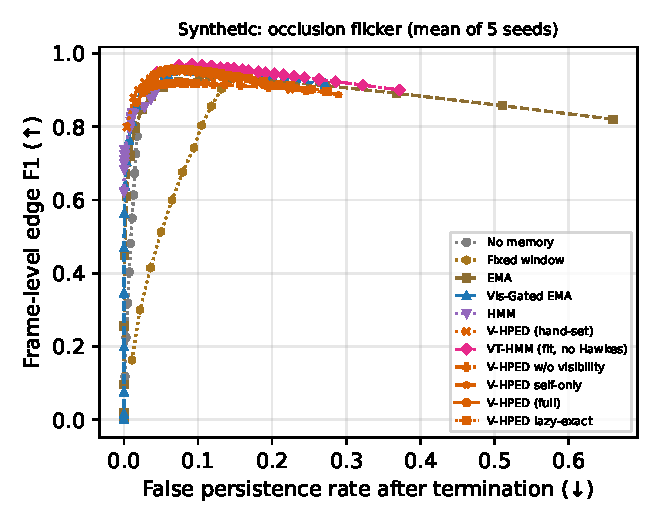
\includegraphics[width=0.48\linewidth]{generated/tradeoff_occlusion_flicker.pdf}
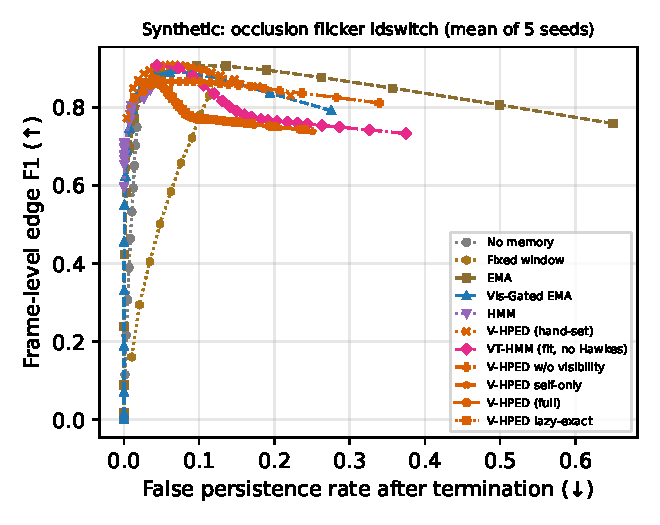
\includegraphics[width=0.48\linewidth]{generated/tradeoff_occlusion_flicker_idswitch.pdf}
\caption{Trade-off curves over thresholds (test, mean over seeds).}
\label{fig:tradeoff}
\end{figure}

\begin{figure}[t]
\centering
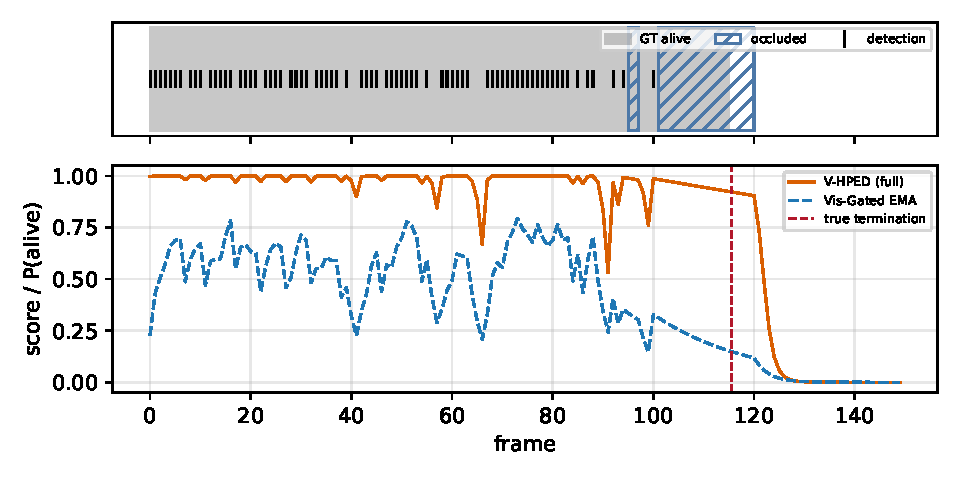
\includegraphics[width=0.9\linewidth]{generated/qualitative.pdf}
\caption{Synthetic example. Top: ground truth, detections, occlusion.
Bottom: alive probability of fitted V-HPED and score of gated EMA.}
\label{fig:qual}
\end{figure}

\begin{figure}[t]
\centering
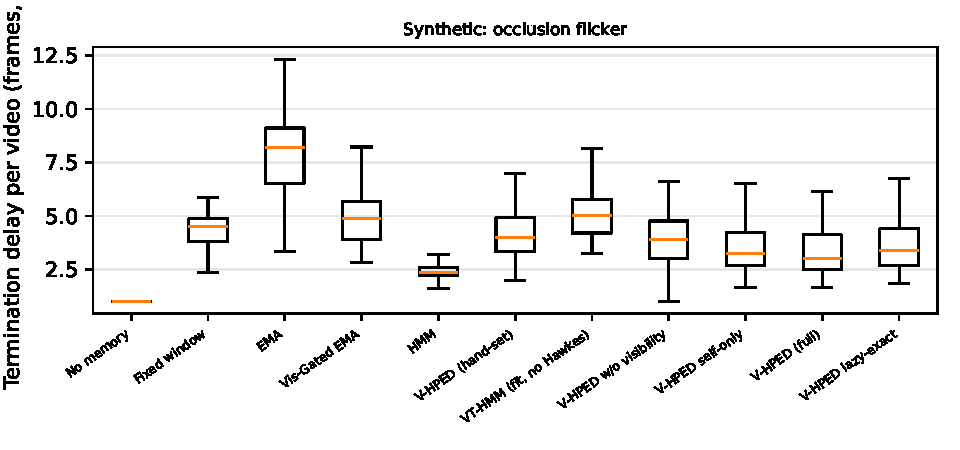
\includegraphics[width=0.48\linewidth]{generated/termination_delay.pdf}
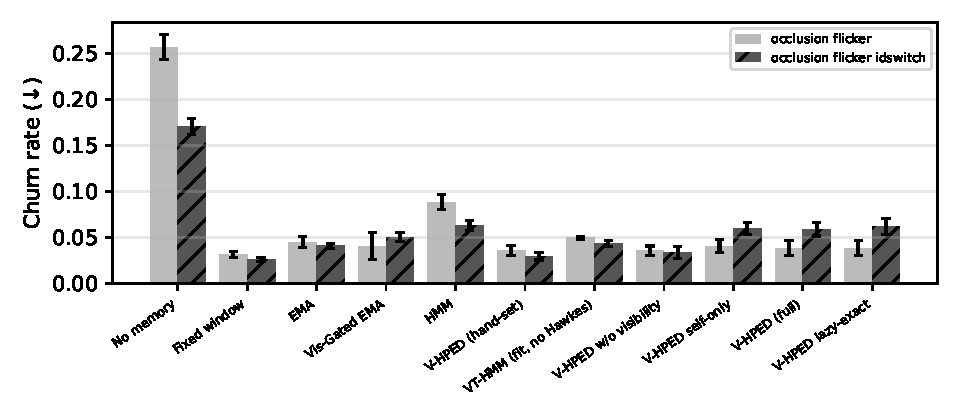
\includegraphics[width=0.48\linewidth]{generated/churn.pdf}
\caption{Termination delay per video and churn.}
\label{fig:delaychurn}
\end{figure}

\subsection{Efficiency of lazy maintenance}
Table~\ref{tab:eff} and Fig.~\ref{fig:eff} compare eager and lazy V-HPED on
traces with $A$ active pairs of which a fraction $f$ have a record in each
frame ($P=26$). Decision mismatches against the eager oracle:
\cxMismatches. With $A=\cxMaxPairs$, lazy is $\cxSpeedupSparse\times$ faster
at $f=\cxFracSparse$, but $\cxSpeedupDense\times$ (i.e.\ slower) at $f=1$,
where nothing can be skipped and scheduling overhead remains. Latency was
measured on \cxMachine; operation counts are machine-independent.

\begin{table}[t]
\centering\scriptsize
\caption{Eager vs.\ lazy per-frame update latency and work.}
\label{tab:eff}
\begin{tabular}{rrrrrr}
\toprule
$f$ & $A$ & eager ms & lazy ms & speed-up & lazy/eager pair updates \\
\midrule
0.05 & 100 & 3.34 & 0.62 & 5.42 & 0.128 \\
0.05 & 300 & 10.08 & 1.86 & 5.41 & 0.128 \\
0.05 & 1000 & 35.54 & 6.49 & 5.48 & 0.125 \\
0.05 & 3000 & 110.87 & 24.87 & 4.46 & 0.125 \\
0.20 & 100 & 3.43 & 1.35 & 2.54 & 0.265 \\
0.20 & 300 & 10.95 & 4.05 & 2.71 & 0.266 \\
0.20 & 1000 & 36.49 & 14.92 & 2.44 & 0.268 \\
0.20 & 3000 & 112.01 & 49.39 & 2.27 & 0.267 \\
0.50 & 100 & 3.45 & 2.70 & 1.28 & 0.546 \\
0.50 & 300 & 10.63 & 8.17 & 1.30 & 0.546 \\
0.50 & 1000 & 37.56 & 28.51 & 1.32 & 0.546 \\
0.50 & 3000 & 114.58 & 91.22 & 1.26 & 0.546 \\
1.00 & 100 & 3.65 & 4.77 & 0.76 & 1.016 \\
1.00 & 300 & 11.80 & 14.43 & 0.82 & 1.016 \\
1.00 & 1000 & 38.77 & 49.43 & 0.78 & 1.016 \\
1.00 & 3000 & 119.23 & 155.82 & 0.77 & 1.016 \\
\bottomrule
\end{tabular}

\end{table}

\begin{figure}[t]
\centering
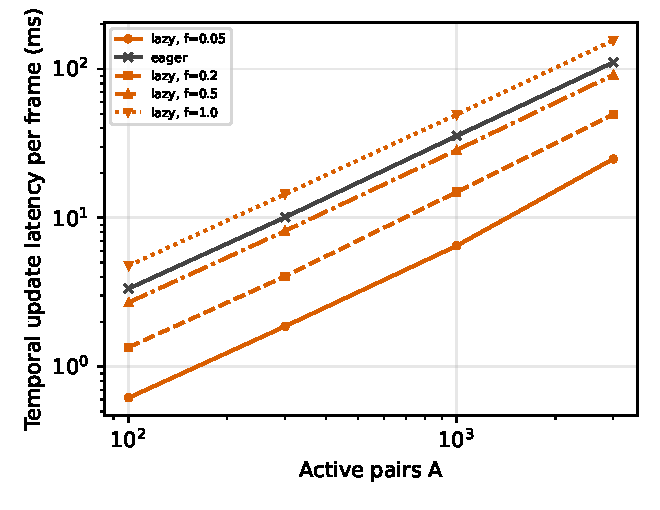
\includegraphics[width=0.45\linewidth]{generated/complexity_latency.pdf}
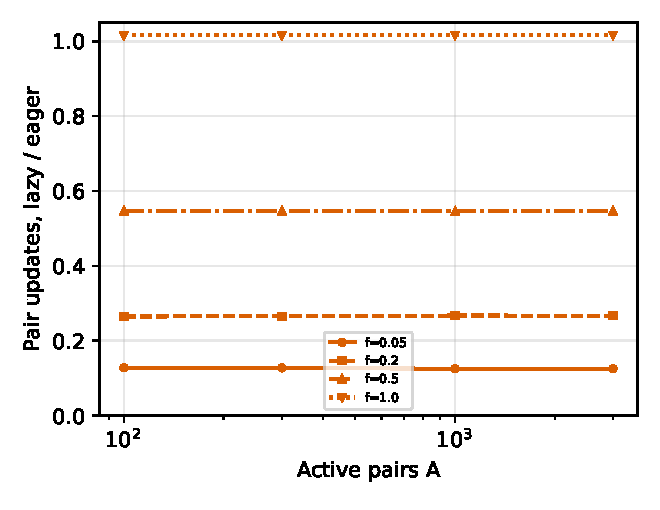
\includegraphics[width=0.45\linewidth]{generated/complexity_work.pdf}
\caption{Latency and pair updates vs.\ active pairs.}
\label{fig:eff}
\end{figure}

\subsection{Action Genome pilot}
\label{sec:pilot}
\ifnum\pilotAvailable=1
\input{generated/pilot_text.tex}
\else
\todo{Not yet run: Action Genome annotations were not available. The
pipeline (loader, format inspection, corruption, fitting, threshold sweep,
hypervolume go/no-go comparisons, figures) is implemented and tested;
run \texttt{scripts/inspect\_action\_genome.py} then
\texttt{scripts/run\_pilot\_ag.py}.}
\fi

\section{Limitations}
\begin{itemize}
\item All quantitative results so far are synthetic or efficiency
benchmarks; no claim about real detectors, trackers or base models is made.
Base-model integration (STTran, DSG-DETR, TEMPURA) and real tracker noise
remain to be run through the frozen adapter contract.
\item Fitted parameters degrade under identity switches: in the synthetic ID-switch
condition the fitted model loses frame F1 to simpler baselines and to its own
hand-set version, and its calibration collapses (Table~
ef{tab:ablid}).
Identity noise creates spurious edges on wrong pairs that unsupervised
likelihood fitting partly absorbs; robust fitting is open.
\item Visibility without Hawkes terms (VT-HMM) attains the best frame F1 in the
flicker condition; the Hawkes terms buy faster termination, not uniformly
higher accuracy.
\item The self-calibrating evidence that speeds up termination also
penalises dense relationships after a few misses, which can increase churn
(Fig.~\ref{fig:qual}, frame $\approx 90$).
\item Lazy evaluation is exact only if absence of a record is fully censored
($\rho_{\textsc{unk}}=0$) and the hazard ignores the traces ($\gamma=0$);
otherwise the implementation falls back to eager updates. Pairs touched
under occlusion are still updated eagerly.
\item Parameters are fitted without alive labels; $\varepsilon$ and
$\lambda$ can trade off (identifiability), so fitted values are interpreted
only through behaviour.
\item Action Genome annotates sparse keyframes; gap lengths are in
annotated frames, and the frozen termination metric also counts
relationships that end because the object becomes invisible.
\end{itemize}

\section{Conclusion}
V-HPED gives temporal scene graphs a principled way to tell an occluded
relationship from one that has ended, and its lazy implementation maintains
it exactly at a cost proportional to the edges that change. Whether the
synthetic advantages hold on real VidSGG predictions is the next,
decisive experiment.

\bibliographystyle{plain}
\bibliography{references}
\end{document}
